%!TEX root = ../thesis.tex

\section{実験概要}
%\begin{figure}[hbtp]
  %\centering
 %\includegraphics[keepaspectratio, scale=0.8]
      %{images/RaspberryPiMouse.png}
 %\caption{Example}
 %\label{Fig:Example}
%\end{figure}
%\subsection{実験概要}
本研究では,本研究室で開発されているロボット ORNE-box3\cite{井口颯人2023屋外自律移動ロボットプラットフォーム-orne} を用いて走行実験を行った.実機ロボットの外観は\figref{Fig:ORNE-box3}に示す.ORNE-box3のセンサ構成については、\figref{Fig:sensor configuration}に示すように,PCとしてJetson Orin NX 16GBを搭載しており、3D LiDAR:R-Fans-16
、IMU:ADIS16465、Encoder : i-Cart middleを備えている.3D LiDARは、自己位置推定と障害物検知に使用し、IMUとエンコーダは、emcl2に対して情報を提供している.

走行ルートは\figref{Fig:Course map of the Tsudanuma Challenge 2025}が示すように,津田沼校舎2号館前から食堂前に設置されたコーンまでとし,
津田沼チャレンジのコースの一部を利用した.このルートは,屋外環境における
自律移動性能を評価するための実環境を想定したものである.


実験では,Navigation2 における各種パラメータを個別に変化させた場合の
ロボットの挙動の変化を調査することを目的とした.
各走行実験においては,対象とするパラメータのみを変更し,
それ以外のパラメータはすべて一定に保った.

また,パラメータの変更に際しては,変更前の設定値を基準値とし,
基準値から増減させた場合のロボットの走行挙動を比較・分析した.
これにより,各パラメータがロボットの走行安定性や挙動に与える影響を
明確にすることを試みた.

\begin{figure}[hbtp]
  \centering
 \includegraphics[keepaspectratio, scale=0.6]
      {images/tsudanumachallenge.png}
 \caption{Course map of the Tsudanuma Challenge 2025(source: \cite{Tsudanumachallenge})}
 \label{Fig:Course map of the Tsudanuma Challenge 2025}
\end{figure}

\begin{figure}[hbtp]
  \centering
 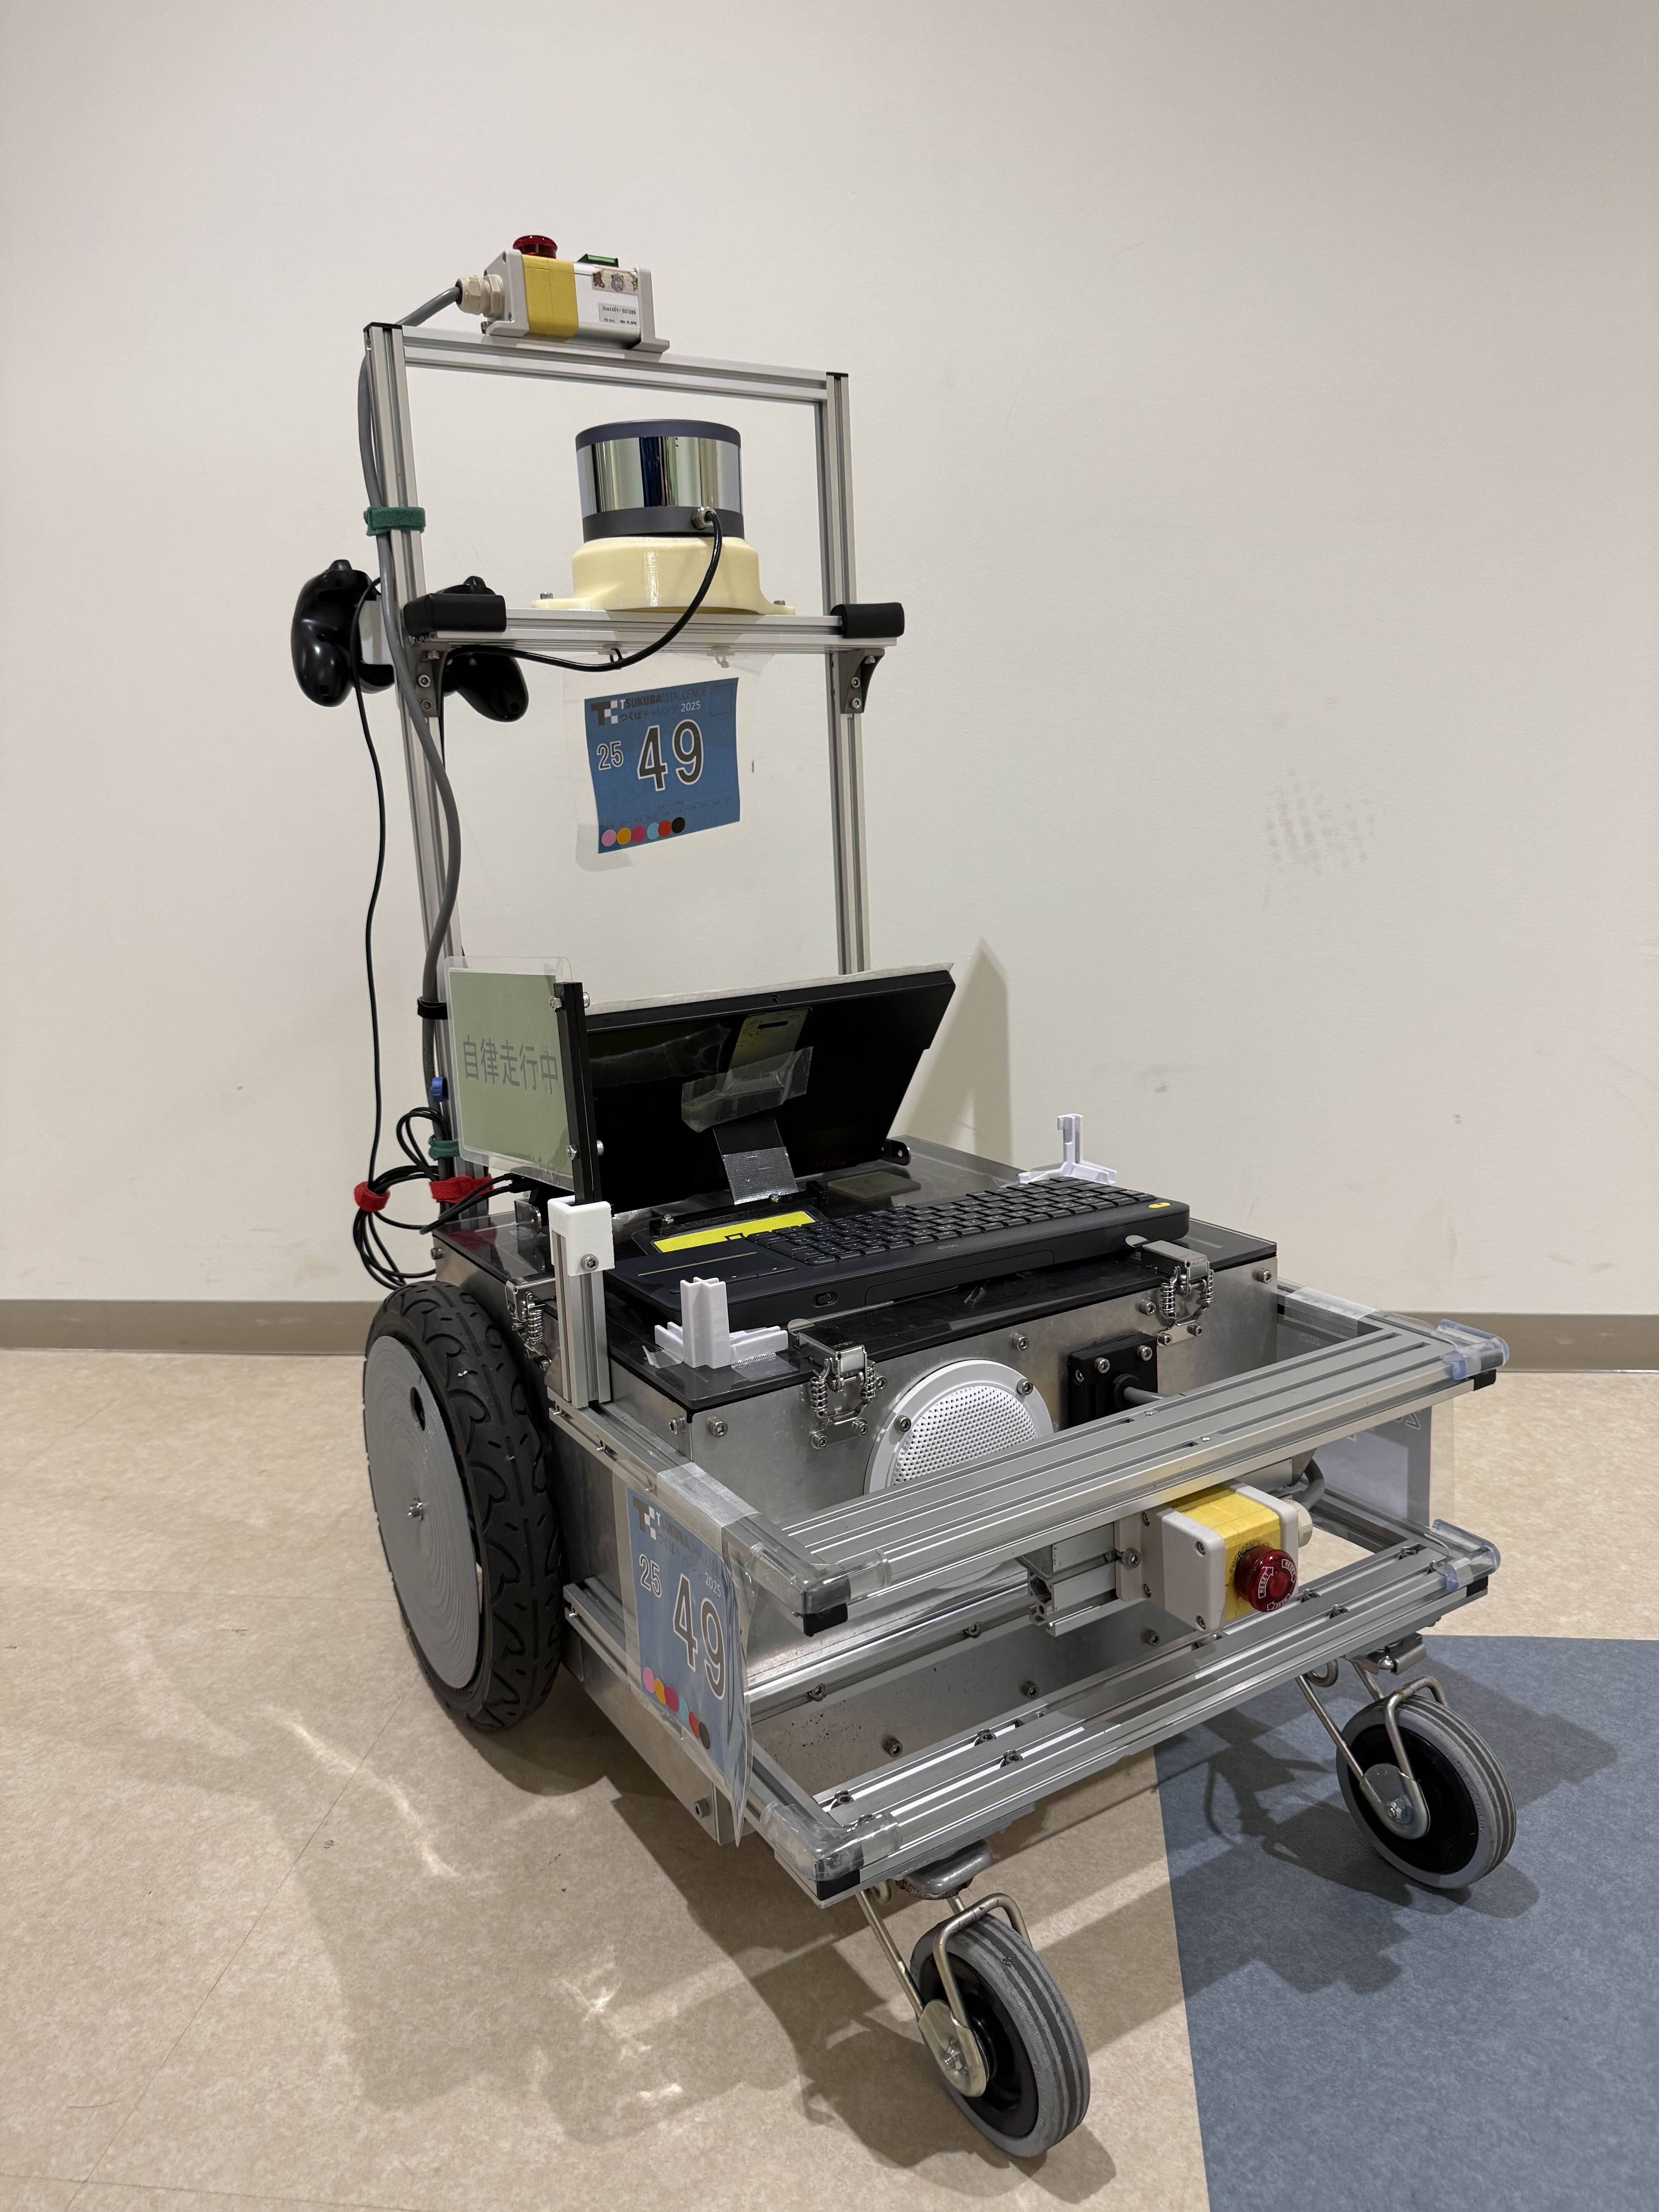
\includegraphics[keepaspectratio, scale=0.3]
      {images/orne-box3.png}
 \caption{ORNE-box3(source: \cite{井口颯人2023屋外自律移動ロボットプラットフォーム-orne})}
 \label{Fig:ORNE-box3}
\end{figure}
\begin{figure}[hbtp]
  \centering
 \includegraphics[keepaspectratio, scale=0.3]
      {images/sensor.png}
 \caption{sensor configuration}
 \label{Fig:sensor configuration}
\end{figure}
%\subsubsection{etc...}






\newpage

\section{実験結果}
%\begin{figure}[hbtp]
  %\centering
 %\includegraphics[keepaspectratio, scale=0.8]
      %{images/RaspberryPiMouse.png}
 %\caption{Example}
 %\label{Fig:Example}
%\end{figure}
\subsection{実験結果(emcl2)}
\subsubsection{実験結果(num\_particles)}

\begin{table}[H]
  \centering
  \caption{パーティクル数の違いによるゴール到達可否}
  \label{tab:num_particles_result}
  \begin{tabular}{c|c|c|c}
    \hline
    & \multicolumn{3}{c}{Number of particles} \\
    \hline
    number of times  & 200 & 500 (base) & 1000 \\
    \hline
    1  & $\times$ & ○ & ○ \\
    2  & ○ & ○ & $\times$ \\
    3  & $\times$ & $\times$ & $\times$ \\
    4  & ○ & ○ & ○ \\
    5  & ○ & ○ & $\times$ \\
    6  & $\times$ & $\times$ & $\times$ \\
    7  & ○ & ○ & ○ \\
    8  & ○ & ○ & ○ \\
    9  & ○ & ○ & ○ \\
    10 & ○ & ○ & ○ \\
    \hline
  \end{tabular}
\end{table}

Table\ref{tab:num_particles_result}に、パーティクル数の違いによるゴール到達の可否を示す.

\begin{table}[H]
  \centering
  \caption{パーティクル数ごとのゴール到達成功率}
  \label{tab:num_particles_success_rate}
  \begin{tabular}{c|c}
    \hline
    パーティクル数 & 成功率 [\%] \\
    \hline
    200  & 60 \\
    500 (base) & 80 \\
    1000 & 60 \\
    \hline
  \end{tabular}
\end{table}

Table\ref{tab:num_particles_success_rate}に,
パーティクル数を変化させた際のゴール到達成功率を示す.

Table\ref{tab:num_particles_result},Table\ref{tab:num_particles_success_rate}が示すように、パーティクル数を 200,500,1000 と変化させて自己位置推定の安定性を評価した.
その結果,パーティクル数 500 の場合に最も高いゴール到達率が得られた.
一方で,200 および 1000 の場合は,到達率がやや低下する傾向が確認された.
パーティクル数が少ないと自己位置推定が破綻しやすく、成功率が低下した.また、パーティクル数が多すぎても計算量の増加によって、遅延が発生して安定性が低下した。
以上より,パーティクル数は多ければ良いわけではなく,
自己位置推定の精度と計算負荷のバランスを考慮した適切な設定が重要であることが分かる.
本実験環境においては,パーティクル数 500 が最も安定した性能を示した.

次からの実験では、\figref{Fig:base direction},\figref{Fig:base position}のグラフが基準の値の時のロボットの挙動である。\figref{Fig:base direction}はロボットの向き、\figref{Fig:base position}はロボットの位置のグラフである。
\begin{figure}[H]
  \centering
 \includegraphics[keepaspectratio, scale=0.65]
      {images/base_muki.png}
 \caption{base orientation}
 \label{Fig:base orientation}
\end{figure}
\begin{figure}[H]
  \centering
 \includegraphics[keepaspectratio, scale=0.5]
      {images/base_postion.png}
 \caption{base position}
 \label{Fig:base position}
\end{figure}

\subsubsection{実験結果(odom\_fw\_dev\_per\_fw)}
基準の値は、0.19
\begin{figure}[H]
  \centering
 \includegraphics[keepaspectratio, scale=0.8]
      {images/fwfwpose.png}
 \caption{Robot orientation with fw\_dev\_per\_fw = 0.01}
 \label{Fig:Robot orientation with fw_dev_per_fw = 0.01 }
\end{figure}
\begin{figure}[H]
  \centering
 \includegraphics[keepaspectratio, scale=0.8]
      {images/fwfwposition.png}
 \caption{Robot position with fw\_dev\_per\_fw = 0.01
}
 \label{Fig:Robot position with fw_dev_per_fw = 0.01}
\end{figure}


\subsubsection{実験結果(odom\_fw\_dev\_per\_rot)}

\subsubsection{実験結果(odom\_rot\_dev\_per\_fw)}

\subsubsection{実験結果(odom\_rot\_dev\_per\_rot)}

\subsubsection{実験結果(laser\_likelihood\_max\_dist)}

\subsubsection{実験結果(range\_threshold)}

\subsection{実験結果(Nav2\_controller)}

\subsubsection{実験結果(max\_vel\_x)}
\subsubsection{実験結果(max\_vel\_theta)}
\subsubsection{実験結果(max\_speed\_xy)}
\subsubsection{実験結果(min\_theta\_velocity\_threshold)}
\subsubsection{実験結果(acc\_lim\_x)}
\subsubsection{実験結果(acc\_lim\_theta)}

\subsection{実験結果(Nav2\_Costmap)}

\subsubsection{実験結果(global\_resolution)}
\subsubsection{実験結果(global\_cost\_scaling\_factor)}
\subsubsection{実験結果(global\_inflation\_radius)}
\subsubsection{実験結果(local\_resolution)}
\subsubsection{実験結果(local\_cost\_scaling\_factor)}
\subsubsection{実験結果(local\_inflation\_radius)}

\subsection{実験結果(Nav2\_Velocity Smoother)}

\subsubsection{実験結果(smoothing\_frequency)}
\subsubsection{実験結果(max\_velocity)}
\subsubsection{実験結果(max\_accel\_ms)}
\subsubsection{実験結果(max\_accel\_rads)}

\subsection{実験結果(Nav2\_planner goal)}

\subsubsection{実験結果(linear\_granularity)}
\subsubsection{実験結果(angular\_granularity)}
\subsubsection{実験結果(xy\_goal\_tolerance)}
\subsubsection{実験結果(trans\_stopped\_velocity)}
\subsubsection{実験結果(planner\_tolerance)}


%\subsubsection{etc...}